\documentclass[11pt, A4paper,norsk]{article}
\usepackage[utf8]{inputenc}
\usepackage[T1]{fontenc}
\usepackage{babel}
\usepackage{amsmath}
\usepackage{amsfonts}
\usepackage{amsthm}
\usepackage{amssymb}
\usepackage[colorlinks]{hyperref}
\usepackage{listings}
\usepackage{color}
\usepackage{hyperref}
\usepackage{graphicx}
\usepackage{cite}
\usepackage{textcomp}
\usepackage{float}

\definecolor{dkgreen}{rgb}{0,0.6,0}
\definecolor{gray}{rgb}{0.5,0.5,0.5}
\definecolor{daynineyellow}{rgb}{1.0,0.655,0.102}
\definecolor{url}{rgb}{0.1,0.1,0.4}

\lstset{frame=tb,
	language=Python,
	aboveskip=3mm,
	belowskip=3mm,
	showstringspaces=false,
	columns=flexible,
	basicstyle={\small\ttfamily},
	numbers=none,
	numberstyle=\tiny\color{gray},
	keywordstyle=\color{blue},
	commentstyle=\color{daynineyellow},
	stringstyle=\color{dkgreen},
	breaklines=true,
	breakatwhitespace=true,
	tabsize=3
}

\lstset{inputpath="C:/Users/Torstein/Documents/UiO/Fys3140/Python programmer"}
\graphicspath{{C:/Users/Torstein/Documents/UiO/Fys3140/"Python programmer"/}}
\hypersetup{colorlinks, urlcolor=url}

\author{Kandidatnummer: 15025}
\title{Svar på Hjemmeeksamen i Fys3140}



%\lstinputlisting{Filnavn! type kodefil}
%\includegraphics[width=12.6cm,height=8cm]{Filnavn! type png}



\begin{document}
\maketitle
	\begin{center}
\includegraphics[scale=1]{{C:/Users/Torstein/Documents/UiO/uio.jpeg}}
	\end{center}
\clearpage
	\begin{center}
\Large \textbf{Oppgaver}
	\end{center}









		\paragraph{1.}
			\begin{gather*}
y'' + \frac{3}{x} y' - \frac{24}{x^2} y = 56 x^6 \\
\text{Hvis vi skal bruke variasjon av parametere for å løse dette trenger vi to} \\
\text{homogene løsninger. En enkel løsning er da å bare teste med potenser av} \\
\text{$x$ siden alle disse $x$ potensene blir like etter derivasjon og deling. Siden vi} \\
\text{har negativ $24$ kan det være naturlig å prøve $x^{4}$, siden $4 \cdot 3$ blir $\frac{24}{2}$ og da} \\
\text{finner vi} \\
(x^4)'' + \frac{3}{x} (x^4)' - \frac{24}{x^2} (x^4) = 0 \\
4 \cdot 3 x^2 + 4 \cdot 3 \frac{1}{x} x^3 - 24 \frac{1}{x^2} x^4 = 0 \\
12x^2 + 12x^2 - 24x^2 = 24x^2 - 24x^2 = 0 \\
\text{Altså er $y_h = Ax^{4}$ en løsning.} \\
\text{En annen løsning kan komme på formen $Bx^{-a}$, og det er naturlig å gjette} \\
\text{på at $a$ skal være lik $6$ siden $6 \cdot 7 = 42$ og $3 \cdot 6 + 24 = 42$} \\
\left( x^{- 6} \right)'' + \frac{3}{x} \left( x^{- 6} \right)' - \frac{24}{x^2} \left( x^{- 6} \right) = 0 \\
(6 \cdot 7) x^{- 8} - ( 3 \cdot 6 ) x^{- 8} - 24 x^{- 8} = 42 x^{- 8} - 18 x^{- 8} - 24 x^{- 8} = 42 x^{- 8} - 42 x^{- 8} = 0 \\
\text{Altså er også $y_h = Bx^{-6}$ en løsning.} \\
\text{Nå har vi to homogene løsninger og kan finne $W$} \\
W = \left|
	\begin{tabular}{ cc }
$x^4$ & $x^{- 6}$ \\
$4x^3$ & $- 6 x^{- 7}$
	\end{tabular}
\right| = - 6 x^{4 - 7} - 4 x^{3 - 6} = - 10 x^{- 3} \\
\text{Da er den partikkulære løsningen gitt ved} \\
y_p = - y_1 \int \frac{y_2 R}{W} dx + y_2 \int \frac{y_1 R}{W} dx \\
y_p = - x^4 \int \frac{x^{-6} 56x^{6}}{- 10x^{-3}} dx + x^{-6} \int \frac{x^{4} 56x^{6}}{- 10x^{- 3}} dx = \frac{56}{10} x^{4} \int x^{3} dx - \frac{56}{10} x^{- 6} \int x^{13} dx \\
y_p = \frac{56}{10} x^{4} \frac{1}{4} x^{4} - \frac{56}{10} x^{- 6} \frac{1}{14} x^{14} = \left( \frac{28 \cdot 14 - 28 \cdot 4}{5 \cdot 4 \cdot 14} \right) x^{8} = x^8 \\
y = y_h + y_p = Ax^{4} + Bx^{-6} + x^{8}
			\end{gather*}





\clearpage
		\paragraph{2.A}
			\subparagraph{a)}
				\begin{flushleft}
$$f(z) = \frac{(z - 2i)^4}{(z - 3 - i)^3}$$
Dette er et utrykk som har en null av rang fire i punktet $z = 2i$ fordi $f(2i) = 0$, og denne nullen er opphøyd i fjerde. Uttrykket har også en tredjeordens pole i $z = 3 + i$ fordi uttryket ikke er definert for dette punktet og når det nærmer seg punktet vil nevneren gå mot null og derfor uttrykket gå mot uendelig. Det er av tredje orden fordi den delen av uttrykket som befinner seg i nevneren og blir null når $z \rightarrow 3 + i$ er opphøyd i tredje.
				\end{flushleft}









			\subparagraph{b)}
				\begin{flushleft}
$$f(z) = \frac{z^3 + 8}{(z - 5)^3(z + 2)} = \frac{(z + 2)(z - 1 - i\sqrt{3})(z - 1 + i\sqrt{3})}{(z - 5)^3(z + 2)}$$
$$f(z) = \frac{(z - 1 - i\sqrt{3})(z - 1 + i\sqrt{3})}{(z - 5)^3}$$
Dette uttrykket har en tredjeordens pole i punktet $z = 5$ og to førsteordens nuller, en i $z = 1 + i \sqrt{3}$ og en i $z = 1 - i \sqrt{3}$.
				\end{flushleft}
			








		\paragraph{2.B}
			\subparagraph{a)}
				\begin{gather*}
f(z) = \frac{P(z)}{Q(z)} \\
g(z) = f(z) \cdot \pi \cot(\pi z) = \frac{f(z) \cdot \pi \cos(\pi z)}{\sin(\pi z)} \\
\text{Siden $f(z)$ er definert og ikke har singuleriteter ved noen $n$ blir residuen} \\
Res(g; n) = \lim_{z \rightarrow n} \frac{f(z) \cdot \pi \cos(\pi z)}{(\sin(\pi z))'} = \frac{f(n) \cdot \pi \cos(\pi n)}{\pi \cos(\pi n)} = f(n)
				\end{gather*}










			\subparagraph{b)}  $ $
				\begin{figure}[H]
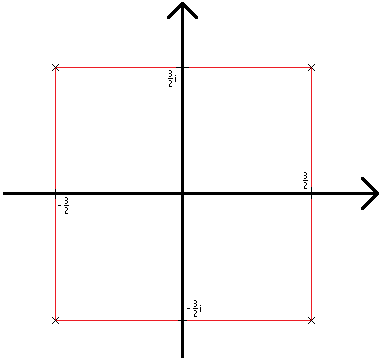
\includegraphics[width=12.6cm,height=9cm]{Skisse_Hjemmeeksamen_2_Bb.png}
\caption{Skisse av kvadratkonturen $\Gamma_N$ med $N = 1$}
				\end{figure}
				\begin{flushleft}
Vi skal se på integralet
$$\lim_{N \rightarrow \infty} \int_{\Gamma_N} g(z) dz = \lim_{N \rightarrow \infty} \int_{\Gamma_N} f(z) \pi \cot(\pi z) dz$$
Vi kan dele integralet inn i to deler, der den ene er integralet langs kurven i det øvre planet, og en annen er integralet i det nedre planet.
$$\lim_{N \rightarrow \infty} \int_{\Gamma_{N}^{+}} f(z) \pi \cot(\pi z) dz + \lim_{N \rightarrow \infty} \int_{\Gamma_{N}^{-}} f(z) \pi \cot(\pi z) dz$$
Fra oppgaveteksten vet vi at det alltid finnes en konstant $M$ som er større enn eller lik $\pi \cot(\pi z)$ altså kan vi si at integralene alltid vil være mindre enn eller lik dette integraler:
$$\lim_{N \rightarrow \infty} \int_{\Gamma_{N}^{+}} f(z) M dz + \lim_{N \rightarrow \infty} \int_{\Gamma_{N}^{-}} f(z) M dz$$
Siden $N \rightarrow \infty$ kan vi se på disse to integralene som integraler langs en bue fra $K$ til $-K$, eller for bua i den negative delen av det komplekse planet fra $-K$ til $K$. Da kan vi endre fra $z$ til $Ke^{i \theta}$, og dermed integrere fra $0$ til $\pi$
$$\lim_{N \rightarrow \infty} \int_{0}^{\pi} f(\theta) M d\theta + \lim_{N \rightarrow \infty} \int_{0}^{- \pi} f(\theta) M d\theta$$
At $N$ går mot uendelig er ekvivalent med at $K$ går mot uendelig i denne situasjonen, så vi kan skrive
$$\lim_{K \rightarrow \infty} \int_{0}^{\pi} f(\theta) M d\theta + \lim_{K \rightarrow \infty} \int_{0}^{- \pi} f(\theta) M d\theta$$
Siden $f(z)$ besto av en brøk med høyere grad i nevner enn i teller vil Den nå inneholde høyere grad av $K$ i nevneren enn i telleren, og siden $K$ går mot uendelig vil $f(\theta)$ gå mot $0$. Dette gjør at hele integralet går mot null, både for buen oppe og nede, og vi får
$$\lim_{N \rightarrow \infty} \int_{\Gamma_N} g(z) dz \leq \lim_{K \rightarrow \infty} \int_{0}^{\pi} f(\theta) M d\theta + \lim_{K \rightarrow \infty} \int_{0}^{- \pi} f(\theta) M d\theta = 0 + 0 = 0$$
				\end{flushleft}








			\subparagraph{c)}
				\begin{gather*}
\frac{1}{2 \pi i} \lim_{N \rightarrow \infty} \int_{\Gamma_N} g(z) dz  = \lim_{N \rightarrow \infty} \sum_{n = - N}^{N} f(n) + \sum( \text{Residuene til $g(z)$ i polene til $f(z)$} ) \\
\text{Fra resultatet over vet vi at venstre side er $0$ og vi får} \\
0 = \lim_{N \rightarrow \infty} \sum_{n = - N}^{N} f(n) + \sum( \text{Residuene til $g(z)$ i polene til $f(z)$} ) \\
\lim_{N \rightarrow \infty} \sum_{n = - N}^{N} f(n) = - \sum( \text{Residuene til $g(z)$ i polene til $f(z)$} )
				\end{gather*}









			\subparagraph{d)}
				\begin{gather*}
\sum_{n = - \infty}^{\infty} \frac{1}{1 + n^2} = \lim_{N \rightarrow \infty} \sum_{n = - N}^{N} f(n) \\
= - \sum ( \text{Residuene til $g(z)$ i polene til $f(z)$} ) = - Res(g; i) - Res(g; - i) \\
= - \lim_{z \rightarrow i} (z - i) g(z) - \lim_{z \rightarrow - i} (z + i) g(z) \\
= - \lim_{z \rightarrow i} (z - i) \frac{1}{(z - i)(z + i)} \pi \cot(\pi z) - \lim_{z \rightarrow - i} (z + i) \frac{1}{(z - i)(z + i)} \pi \cot(\pi z) \\
= - \lim_{z \rightarrow i} \frac{1}{z + i} \pi \cot(\pi z) - \lim_{z \rightarrow - i} \frac{1}{z - i} \pi \cot(\pi z) \\
= - \frac{1}{2i} \pi \frac{i(e^{- \pi} + e^{\pi})}{e^{- \pi} - e^{\pi}} + \frac{1}{2i} \pi \frac{i(e^{\pi} + e^{-\pi})}{e^{\pi} - e^{- \pi}} \\
= - \frac{1}{2} \pi \frac{e^{- \pi} + e^{\pi}}{e^{- \pi} - e^{\pi}} + \frac{1}{2} \pi \frac{e^{\pi} + e^{-\pi}}{e^{\pi} - e^{- \pi}} = \frac{1}{2} \pi \frac{e^{- \pi} + e^{\pi}}{- e^{- \pi} + e^{\pi}} + \frac{1}{2} \pi \frac{e^{\pi} + e^{-\pi}}{e^{\pi} - e^{- \pi}} \\
= \pi \frac{e^{- \pi} + e^{\pi}}{e^{\pi} - e^{- \pi}} = \pi \coth(\pi)
				\end{gather*}











\clearpage
		\paragraph{3.}
			\subparagraph{a)}
				\begin{gather*}
\int_{- \infty}^{\infty} \delta(f(t)) g(t) dt \\
\text{Deler opp i integraler som hver inneholder en $t_i$. Det vil si at $t_{0} + \epsilon_{0} =\equiv - \infty$} \\
\text{og at $t_{\text{siste} + 1} - \epsilon_{siste + 1} \equiv \infty$. I tillegg definerer jeg $\epsilon_{i \pm 1}$ til å være verdien som,} \\
\text{lagt sammen med $t_{i - 1}$ eller trukket fra} \\
\text{$t_{i + 1}$, gjør at jeg kommer midt mellom intervallene i det tallet den er lagt til} \\
\text{eller trukket fra og $t_i$. Altså er det det samme integralet når alt er lagt sammen.} \\
\sum_{i} \int_{t_{i - 1} + \epsilon_{i + 1}}^{t_{i + 1} - \epsilon_{i - 1}} \delta(f(t)) g(t) dt \\
\text{Taylorutvikler $f(t)$ i alle $t_i$, men trenger bare ta med førsteordensleddet siden} \\
\text{jeg bare skal bruke det i punktet $t_i$ uansett.} \\
T_{f}(t_i) = \frac{f(t_i)}{0!} (t - t_i)^{0} + \frac{f'(t_i)}{1!} (t - t_i)^{1} = f(t_i) + f'(t_i) (t - t_i) = f'(t_i) (t - t_i) \\
\text{Vi bytter ut $f(t)$ med $T_{f}(t_i)$ siden deltafunksjonen vil plukke ut disse uansett} \\
\sum_{i} \int_{t_{i - 1} + \epsilon_{i + 1}}^{t_{i + 1} - \epsilon_{i - 1}} \delta(f'(t_i) (t - t_i)) g(t) dt \\
\text{Fra Boas, kapittel 8 har vi, i følge $(11.19)$ at dette blir lik} \\
\sum_{i} \int_{t_{i - 1} + \epsilon_{i + 1}}^{t_{i + 1} - \epsilon_{i - 1}} \frac{1}{|f'(t_i)|}\delta(t - t_i) g(t) dt = \int_{- \infty}^{\infty} \sum_{i} \frac{1}{|f'(t_i)|}\delta(t - t_i) g(t) dt \\
\text{Setter opp det vi startet med, lik det vi endte med} \\
\int_{- \infty}^{\infty} \delta(f(t)) g(t) dt = \int_{- \infty}^{\infty} \sum_{i} \frac{1}{|f'(t_i)|}\delta(t - t_i) g(t) dt \\
\text{og får at da må} \\
\delta(f(t)) = \sum_{i} \frac{1}{|f'(t_i)|}\delta(t - t_i)
				\end{gather*}









			\subparagraph{b.i)}
				\begin{gather*}
\text{Antar det er meningen at jeg skal skrive et uttrykk for $\delta(f(t))$.} \\
\delta(f(t)) = \delta(t^2 - a^2) \\
\text{$f(t)$ har nullpunkt i $t = a$ og $t = - a$} \\
\delta(t^2 - a^2) = \frac{1}{|2a|} \delta(t - a) + \frac{1}{|- 2a|} \delta(t + a) = \frac{\delta(t - a) + \delta(t + a)}{2a}
				\end{gather*}












			\subparagraph{b.ii)}
				\begin{gather*}
\text{Samme antagelse som i forrige oppgave} \\
\delta(f(t)) = \delta(\sin(t)) \\
\text{$f(t)$ har nullpunkt i $t = k\pi$, der $k = 0, 1, 2, \dots$} \\
\delta(\sin(t)) = \sum_{i} \frac{1}{|\cos(k_i\pi)|} \delta(t - k_i\pi) \\
\text{For alle $k_i \pi$ blir $|\cos(k_i \pi)| = 1$} \\
\delta(\sin(t)) = \sum_{i} \delta(t - k_i\pi)
				\end{gather*}












\clearpage
			\subparagraph{c)} $ $
				\begin{figure}[H]
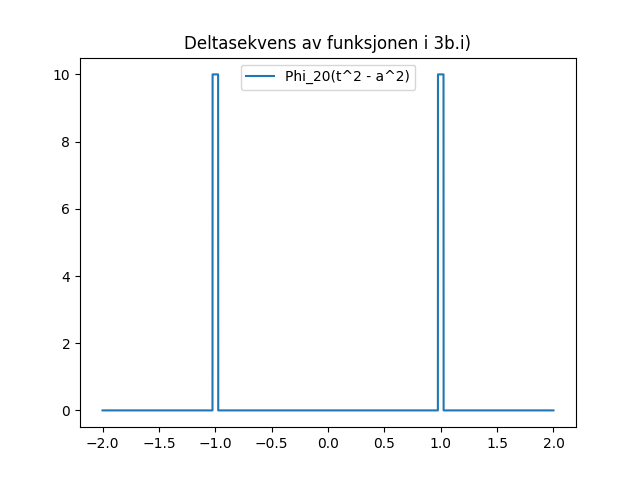
\includegraphics[width=12.6cm,height=7.1cm]{Figur_HE_1.png}
\caption{Plott av delta-sekvens funksjonen $\phi_n(f(t)) = \{ 0 \text{ if } |f(t)| \geq \frac{1}{n} \vee \frac{n}{2} \text{ if } f(t) \leq \frac{1}{n} \}$, med $f(t) = t^2 - a^2$}
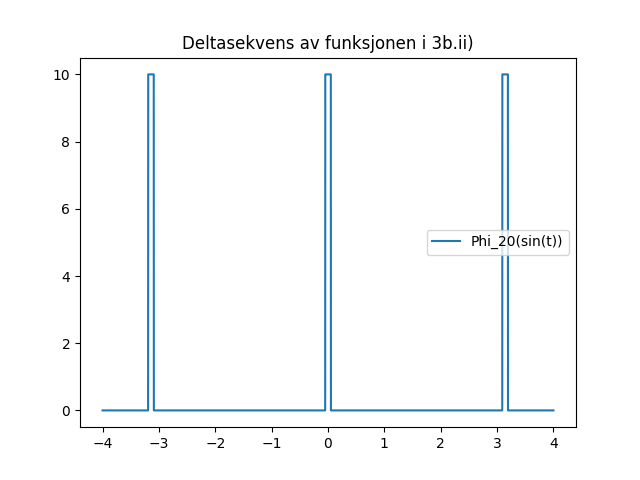
\includegraphics[width=12.6cm,height=7.1cm]{Figur_HE_2.png}
\caption{Plott av delta-sekvens funksjonen $\phi_n(f(t)) = \{ 0 \text{ if } |f(t)| \geq \frac{1}{n} \vee \frac{n}{2} \text{ if } f(t) \leq \frac{1}{n} \}$, med $f(t) = \sin(t)$}
				\end{figure}
				\begin{flushleft}
Ser at deltafunskjonen trekker ut nullpunktene til funksjonen, akkurat sånn som forventet.
\lstinputlisting{Hjemmeeksamen_3c.py}
				\end{flushleft}







			\subparagraph{d)}
				\begin{gather*}
\int_{- \frac{\pi}{2}}^{\frac{\pi}{2}} \cos(t) \delta(\sin(t)) dt \\
\text{Bruker uttrykket fra $3. b.ii)$} \\
\int_{- \frac{\pi}{2}}^{\frac{\pi}{2}} \cos(t) \sum_{i} \delta(t - k_i\pi) dt = \int_{- \frac{\pi}{2}}^{\frac{\pi}{2}} \cos(t) \delta(t - 0) dt = \cos(0) = 1 \\
\int_{- \frac{\pi}{2}}^{\frac{\pi}{2}} \cos(t) \delta(\sin(t)) dt = 1
				\end{gather*}
\end{document}